In this section we will describe the datasets used, the data engineering
pipeline, including pre-processing and feature extraction, the speaker
recognition models evaluated and the adversarial attacks investigated in this paper.

\subsection{Datasets}
In our experiments we use three datasets, each assigned to a model as described
in Table\ref{tbl:datasets}. The datasets used are public and provide audio clips
of different lengths, quality, language and content.

\begin{table}[!h]
\centering
\begin{tabular}{llllll}
                                                                     & \cellcolor[HTML]{C0C0C0}Speakers & \cellcolor[HTML]{C0C0C0}Language & \cellcolor[HTML]{C0C0C0}Duration & \cellcolor[HTML]{C0C0C0}Context & \cellcolor[HTML]{C0C0C0}Model \\ \cline{2-6} 
\multicolumn{1}{l|}{\cellcolor[HTML]{C0C0C0}2013 Blizzard} & 1                                & English                          & 73 h                             & Book narr.                  & SampleRNN                     \\
\multicolumn{1}{l|}{\cellcolor[HTML]{C0C0C0}CSTR VCTK}               & 109                              & English                          & 400 Sentences                    & Newspaper ++               & WaveNet                       \\
\multicolumn{1}{l|}{\cellcolor[HTML]{C0C0C0}2004 NIST}               & 100                              & Multiple                         & 5 min / speaker                  & Conversational tel. & WGAN                         
\end{tabular}
\bigskip
\caption{Description of datasets used in our experiments. Book narr. refers to
    book narrations. Newspaper ++ refers to newspapers and other documents.
    Conversational tel. refers to conversational telephone speech.}
\label{tbl:datasets}
\end{table}

\subsection{Pre-processing}
\label{sub:processdata}
Data pre-processing is dependent on the model being trained. For SampleRNN and
WaveNet, the raw audio is reduced to 16kHz and quantized using the $\mu-law$
companding transformation as referenced in SampleRNN~\cite{mehri2016samplernn}
and WaveNet~\cite{van2016wavenet}. For the model based on the Wasserstein GAN,
we pre-process the data by converting it to 16kHz and removing silences by using
the WebRTC Voice Activity Detector (VAD) as referenced
in~\cite{zeidan2014webrtc}. For the speaker recognition system, the data is
pre-processed by converting it to 16kHz when necessary and removing silences by
using the aforemetioned VAD. 

\subsection{Feature extraction}
SampleRNN and WaveNet operate at the sample level, i.e. waveform, thus requiring
no feature extraction.  The features used for the neural speaker recognition
system is based on Mel-Spectrograms with dynamic range compression. The
Mel-Spectrogram is obtained by projecting a spectrogram onto a mel scale. We use
the python library librosa~\cite{mcfee2015librosa} to project the spectrogram
onto 64 mel bands, with window size equal to 1024 samples and hop size equal to
160 samples, i.e. frames of 100ms long. Dynamic range compression is computed as
described in~\cite{lukic2016speaker}, with $log(1 + C*M)$, where $C$ is the a
compression constant scalar set to $1000$ and $M$ is the matrix representing the
Mel-Spectrogram. The speaker recognition system operates on the Mel-Spectrogram
with dynamic range compression as previously described.
                        
\subsection{Neural speaker recognition system}
\label{sub:speaker_recognition}
The speaker recognition system used in our experiments is based on the state-of-the-art framework by \cite{lukic2016speaker} and is described in Figure \ref{fig:CNN}. The first module at the bottom is a pre-processing step that extracts Mel-Spectrogram from the waveform as described in section \ref{sub:processdata}. The second module is a convolutional neural network (CNN) that performs multi-speaker classification using the Mel-Spectrogram. The CNN is a modified version of Alexnet~\cite{krizhevsky2012imagenet}.

\begin{figure}[h]
    \centering
    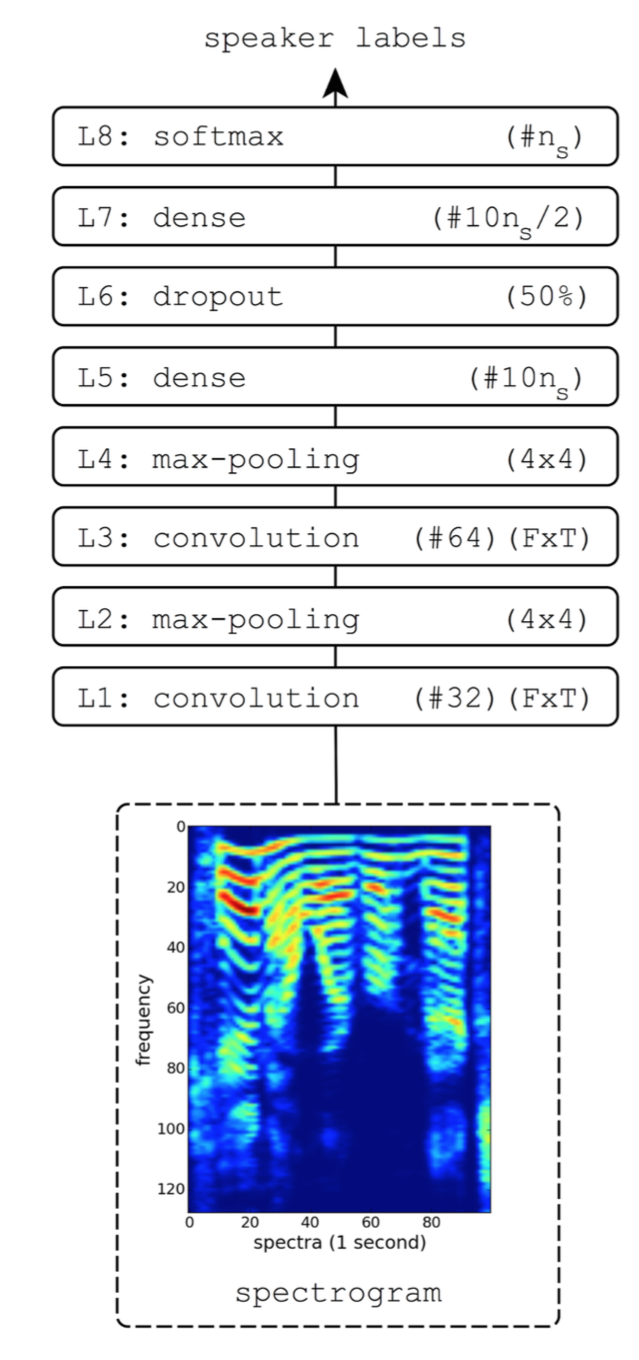
\includegraphics[width=0.25\textwidth]{./fig/cnn.png}
    \caption{Architecture for CNN speaker verifier}
    \label{fig:CNN}
\end{figure}

We train the CNN on our training set using 64*64 Mel-Spectrograms~\footnote{64 mel bands and 64 frames, 100 ms each} consisting of balanced samples from 101 speakers from the NIST 2004 and Blizzard datasets. Our model achieves 85\% test set accuracy.

\section{Adversarial attacks}
We define adversarial attacks on speaker recognition systems as targeted or untargeted. In
targeted attacks, an adversary is interested in designing an adversarial input
that makes the classification system predict a target class chosen by the
adversary. In untargeted attacks, the adversary is interest in a confident
prediction, regardless of the class being predicted. In the following section we
describe our results using targeted and untargeted attacks using existing
generative methods (WaveNet and sampleRNN) and using the GAN framework.
